% ---------------------------------------------------------------------------- %
\begin{figure}
  \centering
	\subfigure[\label{fig:results:giallo:complex:glasses}]
	{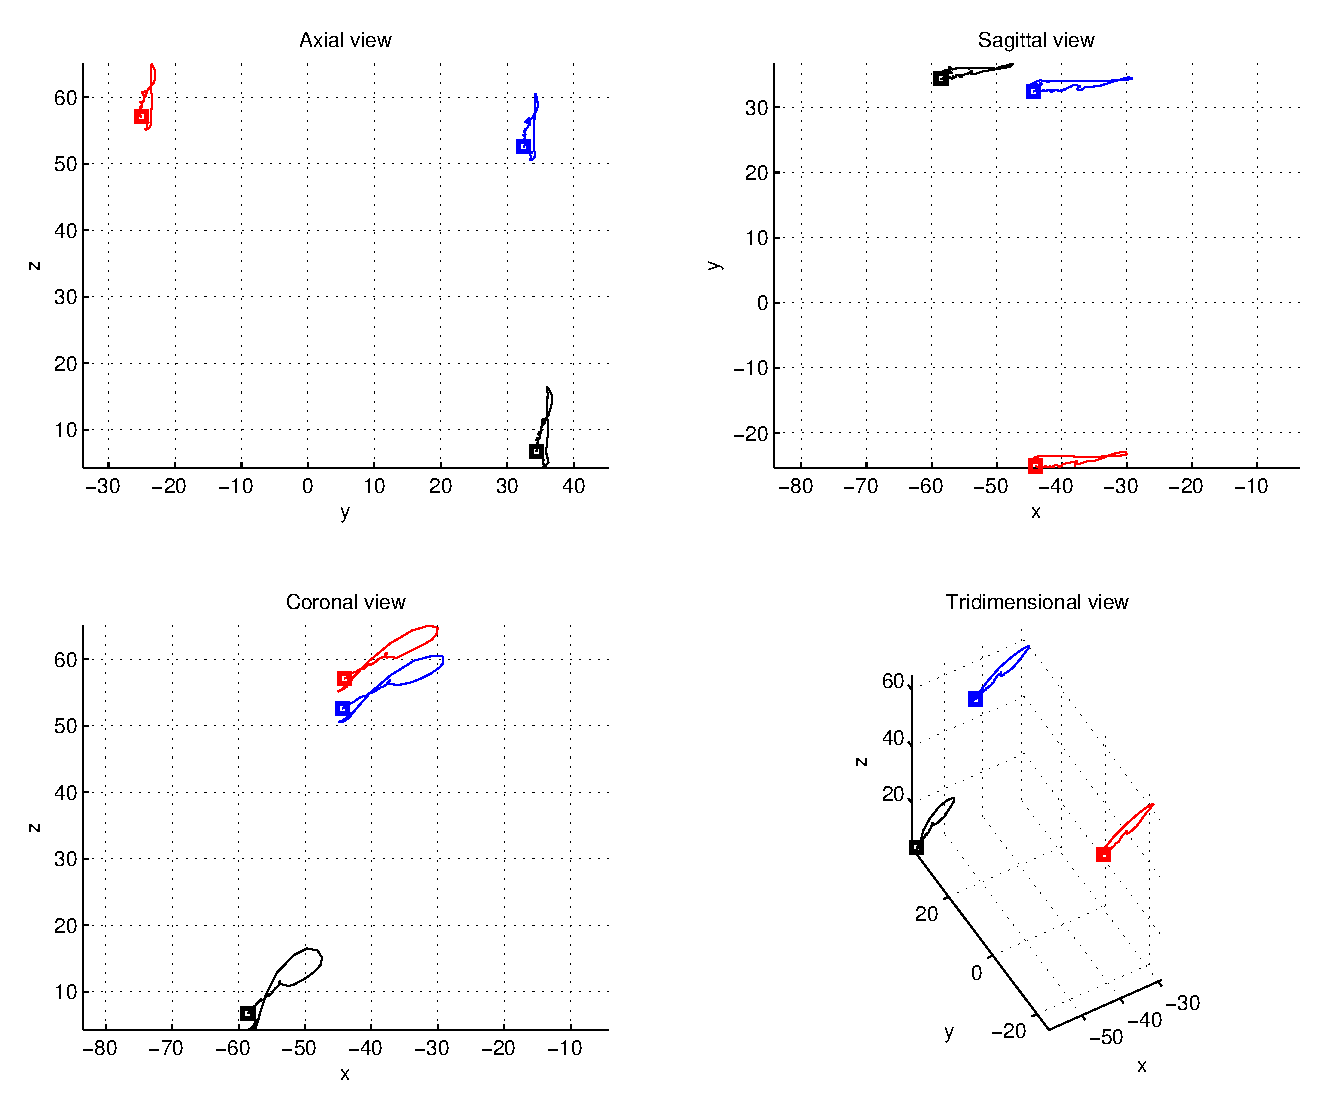
\includegraphics[width=0.45\textwidth]{include/results/images/complex_20_glasses.eps}}
	\hspace{0.05\textwidth}
	\subfigure[\label{fig:results:giallo:complex:tongue}]
	{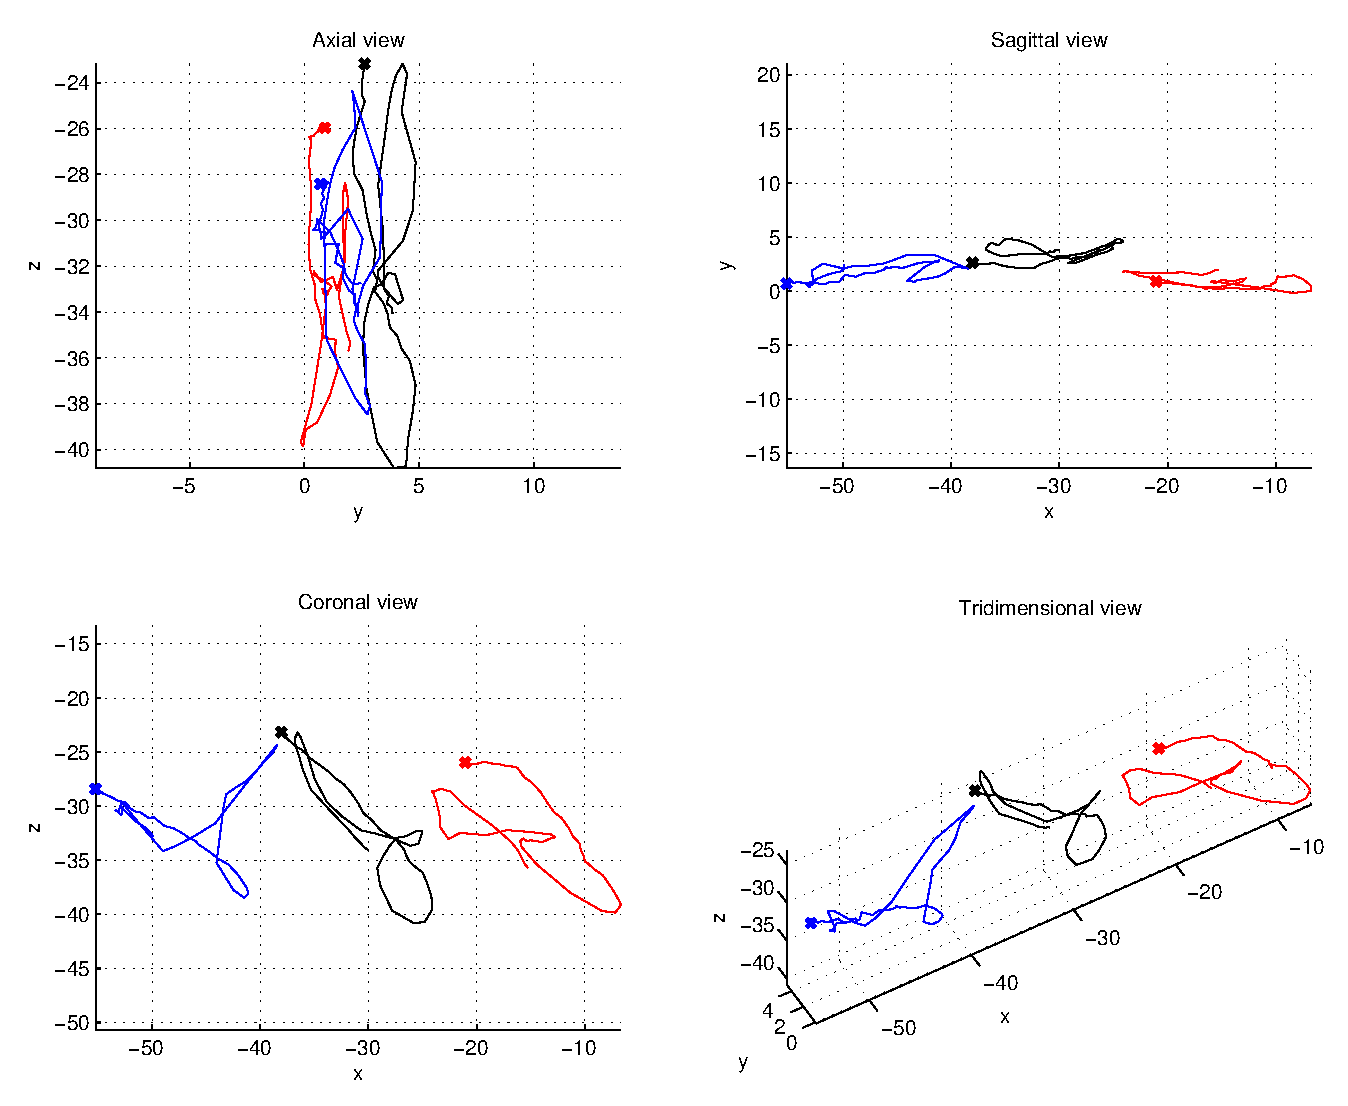
\includegraphics[width=0.45\textwidth]{include/results/images/complex_20_tongue.eps}}

	\caption[Projections of the trajectories of few sensors for /giallo/]{\textbf{Projections of the trajectories of few sensors for /giallo/}: 
	the reader should refer to the caption of
	Figure~\ref{fig:results:uovo:complex}.
	Note: (a) sensor 10 in blue, sensor 11 in red and sensor 12 in black; 
	(b) sensor 1 in red, sensor 2 in black and sensor 3 in blue.
	This plot adheres to the convention shown in 
	Figure~\ref{fig:experiments:map}.
	The thick marks indicate the final position of the sensors.
	}
	\label{fig:results:giallo:complex}
\end{figure}
% ---------------------------------------------------------------------------- %
